\chapter{Prototype Implementation}
\label{cha:implementation}
\vspace{0.4 cm}

This chapter presents which components of the system have been implemented and how.
Only a subset of the components of the designed architecture in chapter~\ref{cha:system} have been implemented.
This is because a prototype was developed as a Proof of Concept (PoC) with a focus on key components for validating the core system functionalities for each specific use case.
These are the training of models, the forecast of new data, and the evaluation of the performance of the developed models.
The remaining components were not implemented since they were not crucial for having a working system, in fact, the overall architecture was designed in order to build a Software as a Service (SaaS) on the implemented core system functionalities.

The first section describes the implementation of the system's common components across the various specific use cases and the others explain the implementation details of the use case-specific modules.
After this chapter, it will be clear how the system prototype was implemented and ready for validation and testing phases, which are discussed in chapter~\ref{cha:evaluation}.


\section{System's common components}
\label{sec:componentsimpl}
\vspace{0.2 cm}

The effectively implemented components of the architecture designed for the proposed system are reported in figure~\ref{fig:implementationcomponents}.
The interactions among them are reported in figure~\ref{fig:implementationinteractions}.

\begin{figure}[H]
\centering
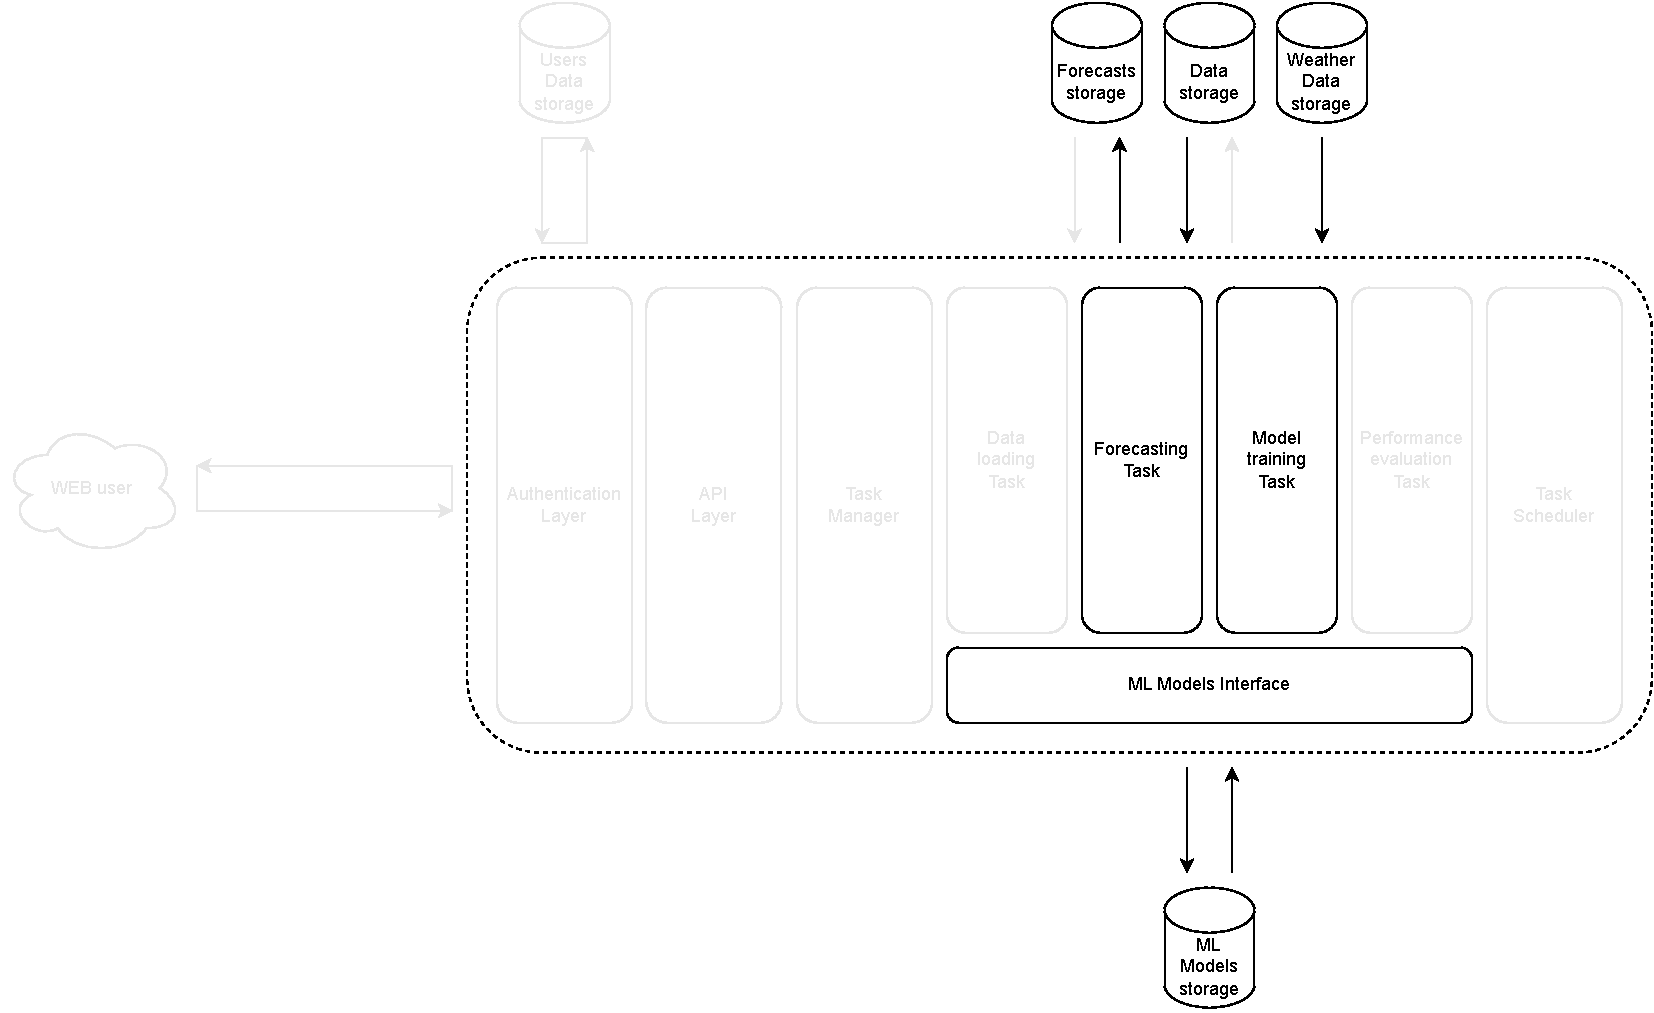
\includegraphics[width=0.9\textwidth]{images/implementation_components}
\caption{The effectively implemented components of the architecture designed for the proposed system.}
\label{fig:implementationcomponents}
\end{figure}

The ML model interface was implemented using the pickle library\footnote{ \url{https://docs.python.org/3/library/pickle.html} } for interfacing with the ML models storage for storing the ML models and retrieving the stored ones making them available for prediction and evaluation.
The use of the MLflow client\footnote{ \url{https://mlflow.org/} } was thought of as a possible interface in the complete system integration for interfacing with the ML models storage.

The model training task trains new models based on available data for the specific use case.
The details about the models and their training process for each specific use case are reported in the dedicated sections.

The forecasting task forecasts future data using the available models for the specific use case.
The details about the models and their forecasting process for each specific use case are reported in the dedicated sections.

The performance evaluation task evaluates the performance of the available models for the specific use case.
The details about the performance evaluation process for each specific use case are reported in chapter~\ref{cha:evaluation}.

\begin{figure}[H]
\centering
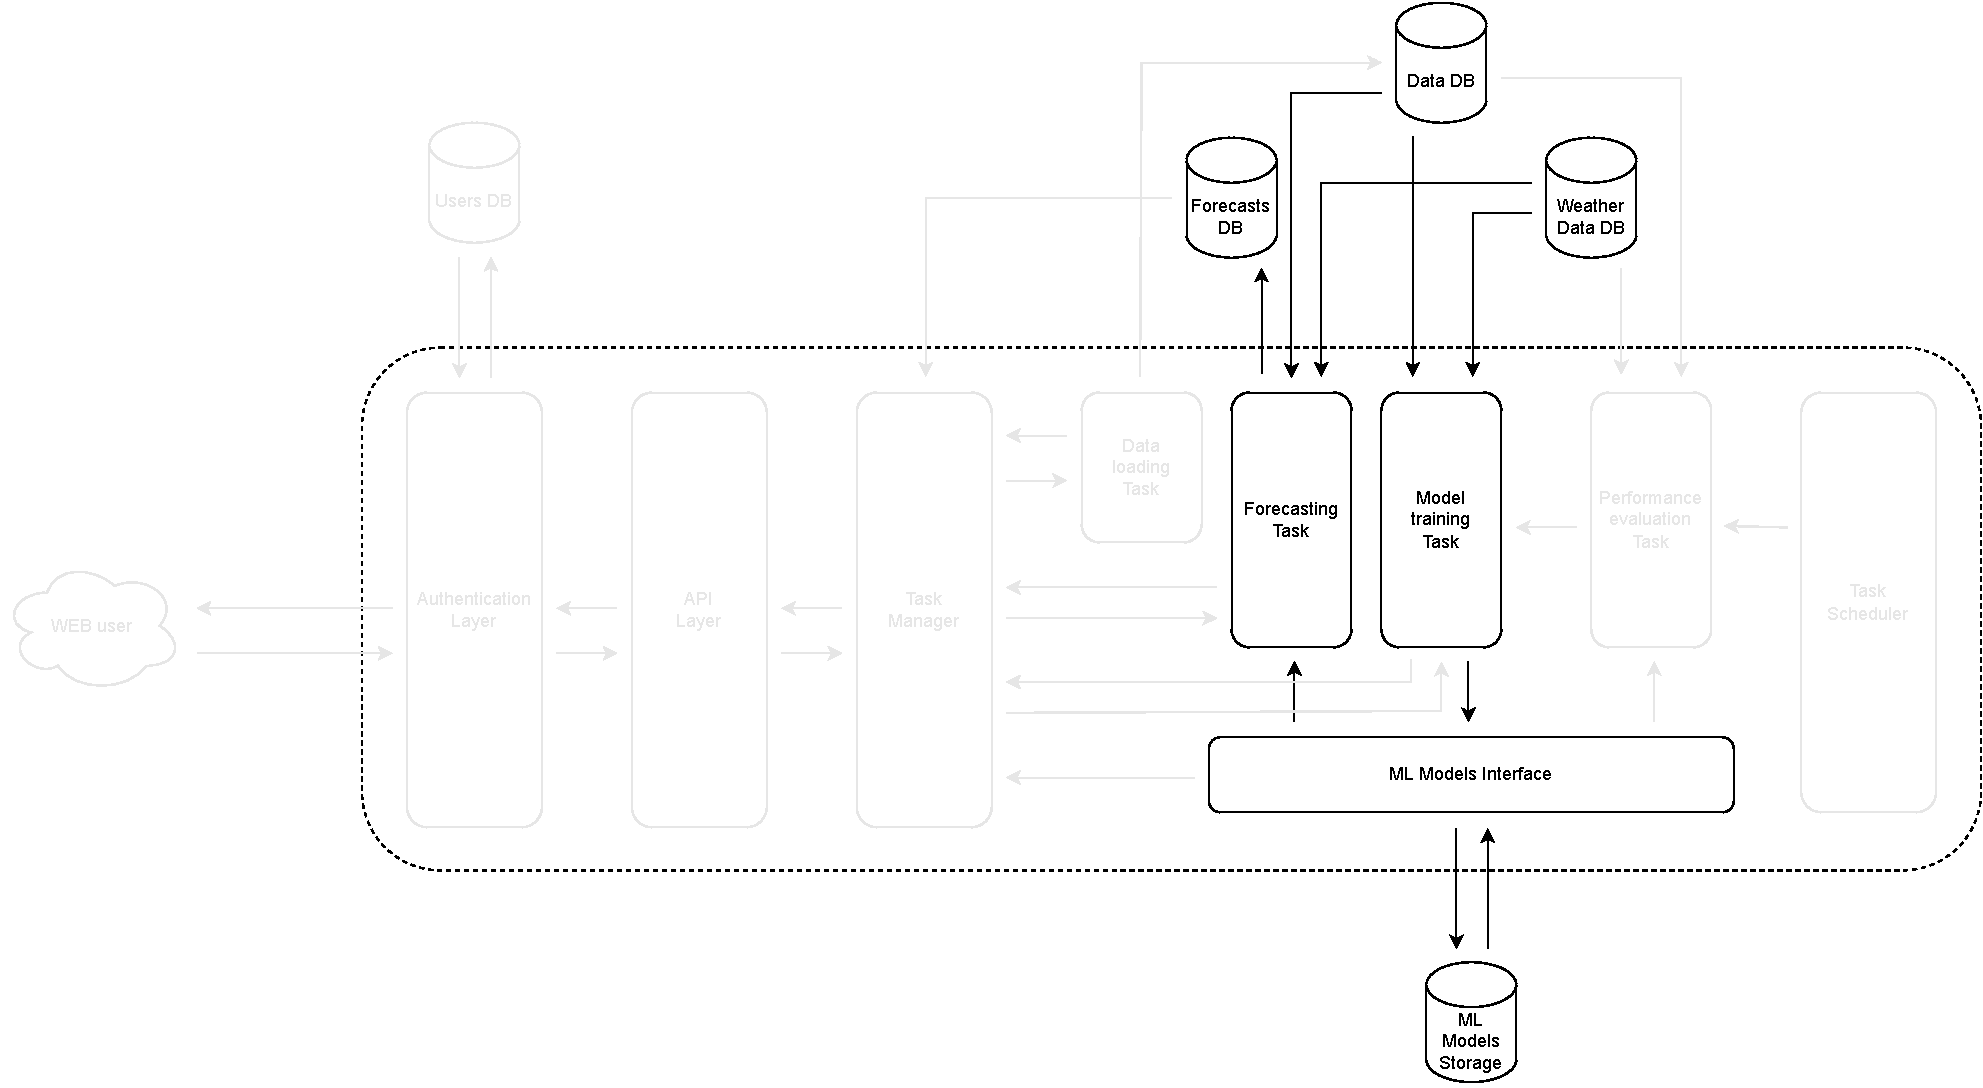
\includegraphics[width=1\textwidth]{images/implementation_interactions}
\caption{The interactions among the effectively implemented components of the architecture designed for the proposed system.}
\label{fig:implementationinteractions}
\end{figure}

The system interacts with the following external components: data storage, weather data storage, ML models storage, and forecasts storage.

The data storage consists of CSV files containing the data for the different use cases, which are loaded using the pandas library\footnote{ \url{https://pandas.pydata.org/} }.
InfluxDB\footnote{ \url{https://www.influxdata.com/} } was thought of as a possible database in the complete system integration for managing the data.

The weather data storage consists of a JSON file containing the weather data, which are loaded using the pandas library.
Weather data is manually obtained from the Weatherbit\footnote{ \url{https://www.weatherbit.io/} } APIs.
InfluxDB was thought of as a possible database in the complete system integration for managing the weather data with an automatic download of weather data using Weatherbit APIs.

The ML models storage consists of pickle files containing the ML models.
MLflow was thought of as a possible ML model storage in the complete system integration for managing the ML models.

The forecasts storage consists of CSV files containing the forecasts, which are stored using the pandas library.
InfluxDB was thought of as a possible database in the complete system integration for managing the forecasts.


\section{Electricity demand forecasting models}
\label{sec:demandimpl}
\vspace{0.2 cm}

The implementation of the electricity demand forecasting models relies on the data preprocessing which consists of parsing the aggregated production data over the customers from a CSV file.
Then, this basic data is enhanced with the air temperature, apparent temperature, and relative humidity parsed from JSON file, in which the reported value is the average of the value in the last hour.
Finally, data is cleaned by filling the gaps by using a linear interpolation, which was effective since there was just some missing data in the weather information.
Two possible granularities were considered: hourly, daily.
Data are already with an hourly granularity, for the daily granularity data are also aggregated over the day summing the consumption of the single hours.


- models training: describe the training for all the specific models;
prediction: describe the prediction for all the specific models.
+ created features that arrive in input to the models -


The developed models are some baseline approaches which consider repeating past days and weeks, an ARIMA model, a hist gradient boosting regressor model, an extreme gradient boosting regressor model, a prophet model, a LSTM model, a GRU model, a CNN model, a combination of the previous techniques, a TFT model, and an AutoML approach.

The ARIMA model was developed using the pmdarima library\footnote{ \url{http://alkaline-ml.com/pmdarima/} }.

The support vector regressor and hist gradient boosting regressor models were developed using the scikit-learn library\footnote{ \url{https://scikit-learn.org/} };

The extreme gradient boosting regressor model was developed using the XGBoost library\footnote{ \url{https://xgboost.readthedocs.io/} };

The prophet model was developed using the prophet library\footnote{ \url{https://facebook.github.io/prophet/} };

The LSTM, GRU, and CNN models were developed using the keras library\footnote{ \url{https://keras.io/} };

The TFT model was developed using the pytorch-forecasting library\footnote{ \url{https://pytorch-forecasting.readthedocs.io/} };

The AutoML approach was based on Auto-PyTorch library\footnote{ \url{https://automl.github.io/Auto-PyTorch/master/} }.


\section{Consumption baseline forecasting models}
\label{sec:baselineimpl}
\vspace{0.2 cm}

Describe the implementation of the consumption baseline forecasting models ...
\begin{itemize}
  \item data preprocessing: consists of parsing single customer consumption data from a CSV file, then basic data is enhanced with the following weather information parsed from JSON file, the reported value is the average of the value in the last hour: air temperature, apparent temperature, and relative humidity. Finally, data is cleaned by filling the gaps by using a linear interpolation;
  \item models training: describe the training for all the specific models;
  \item prediction: describe the prediction for all the specific models.
\end{itemize}


 - TODO describe what the models take in input for training/forecasting (or maybe in chapter 5) -


The developed models are the following: some baseline approaches which consider repeating past days and weeks, an ARIMA model, a hist gradient boosting regressor model, an extreme gradient boosting regressor model, a prophet model, a LSTM model, a GRU model, a CNN model, a combination of the previous techniques, a TFT model, and an AutoML approach.

The ARIMA model was developed using the pmdarima library.
The support vector regressor and hist gradient boosting regressor models were developed using the scikit-learn library;
The extreme gradient boosting regressor model was developed using the XGBoost library;
The prophet model was developed using the prophet library;
The LSTM, GRU, and CNN models were developed using the keras library;
The TFT model was developed using the pytorch-forecasting library;
The AutoML approach was based on Auto-PyTorch.


\section{Electricity production forecasting models}
\label{sec:productionimpl}
\vspace{0.2 cm}

Describe the implementation of the electricity production forecasting models ...
\begin{itemize}
  \item data preprocessing: consists of parsing single PV plant production data from a CSV file, aggregating the single PV plant data to obtain the aggregated production data over the PV plants, then basic data is enhanced with the following weather information parsed from JSON file, the reported value is the average of the value in the last hour: air temperature, apparent temperature, relative humidity, wind speed, wind direction, pressure altimeter, visibility, sky coverage, diffuse horizontal irradiance, direct normal irradiance, global horizontal irradiance, solar radiation, UV index, solar elevation angle, and solar azimuth angle. Finally, data is cleaned by filling the gaps by using a linear interpolation;
  \item models training: describe the training for all the specific models;
  \item prediction: describe the prediction for all the specific models.
\end{itemize}


 - TODO describe what the models take in input for training/forecasting (or maybe in chapter 5) -


The developed models are the following: some baseline approaches which consider repeating past days and weeks, an ARIMA model, a hist gradient boosting regressor model, an extreme gradient boosting regressor model, a prophet model, a LSTM model, a GRU model, a CNN model, a combination of the previous techniques, a TFT model, and an AutoML approach.

The ARIMA model was developed using the pmdarima library.
The support vector regressor and hist gradient boosting regressor models were developed using the scikit-learn library;
The extreme gradient boosting regressor model was developed using the XGBoost library;
The prophet model was developed using the prophet library;
The LSTM, GRU, and CNN models were developed using the keras library;
The TFT model was developed using the pytorch-forecasting library;
The AutoML approach was based on Auto-PyTorch.
